\chapter{Progressions}

Figure~\ref{iiprog} presents one of the most common truisms circulated regarding jazz harmony in a new form.  Each of the curves plotted here describes the statistical behavior of a chord category following the appearance of a locally-transposed\footnote{I explain the complexities of the (novel) key-finding algorithm in Chapter 6.  In short, the algorithm assembles pitch class profiles for a wide variety of sliding window sizes for each solo track.  It then calculates the average perplexity of the pitch class profile for each possible window size and compares it to the perplexity of pitch class key profiles commonly employed in the literature.  When a particular window size yields profile perplexities close to that of the Bellman-Budge key profile, the algorithm assumes this is the right time scale for key-finding; it slides the chosen window through a given track and assigns a best-guess local key to each chord.  All chords are then transposed relative to their local key, yielding semitonal scale degree sets in place of pitch class sets.} $ii$ chord.  The details of Figure~\ref{iiprog} will emerge below, but the general form of the plot is simple: the vertical axis gives a measure of probability, while the horizontal displays time elapsed after $ii$.  Each curve tracks the probability of a particular chord appearing after $ii$ over time.

\begin{figure}
	\centering
	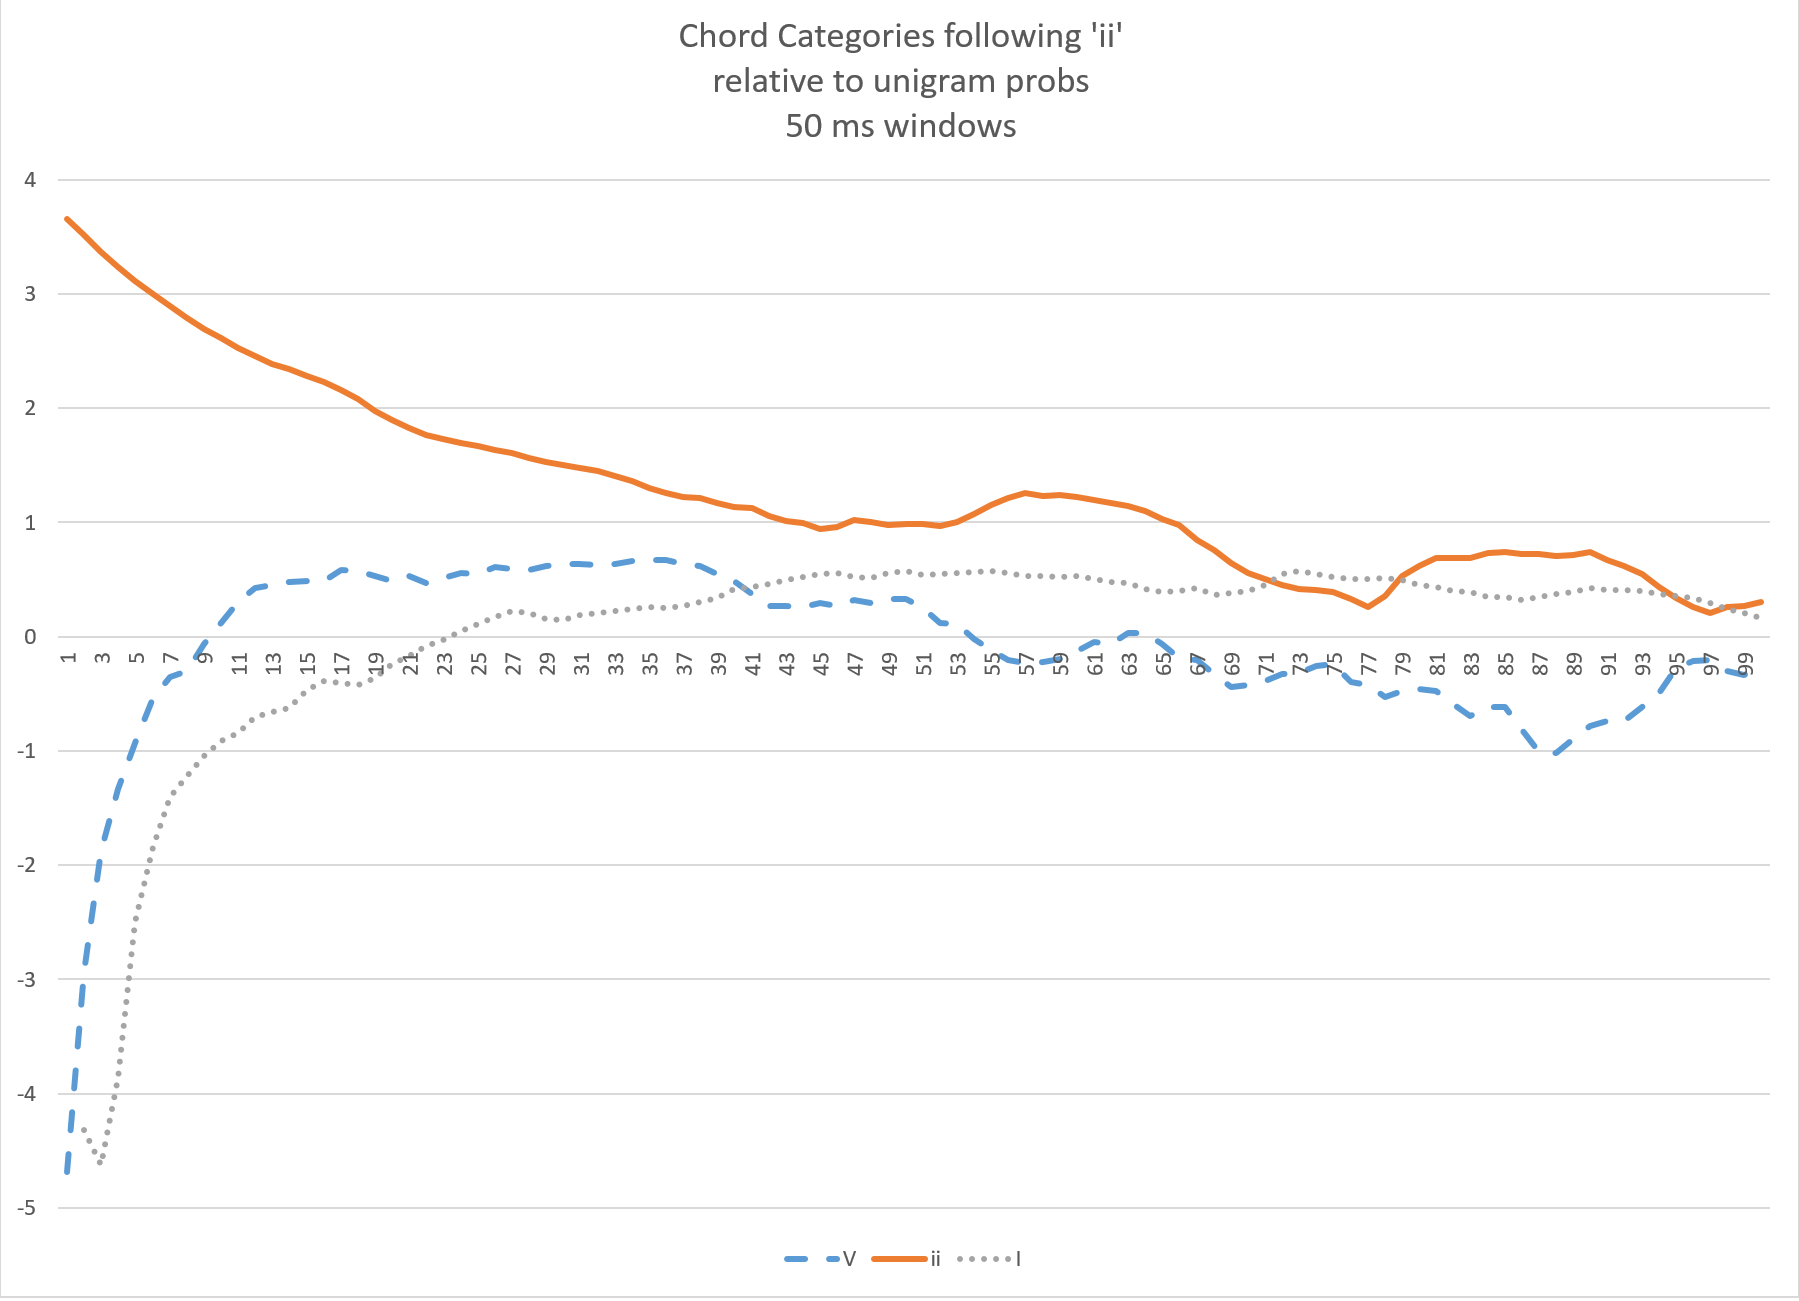
\includegraphics[width=5.5in]{iiprogressions.png}
	\caption{The unigram-relative log probabilities of $ii$ (red line), $V$ (blue line), and $I$ (gray line) versus time elapsed after a $ii$ chord in the YJaMP corpus.  Horizontal axis values are consecutive 50-millisecond time windows.  Here, the categories for $V$, $ii$, and $I$ have been hand-chosen; Chapter 5 provides a means to bootstrap category formation.}
	\label{iiprog}
\end{figure}

The truism: in jazz, $ii$ often progresses to $V$ and then to $I$.  The curves of Figure~\ref{iiprog} have different shapes -- different behaviors over time -- which might be said to demonstrate the truism in explicitly temporal terms.  The (blue, dashed) curve for $V$ rises to a probability peak between time points 17 and 37, after which it slowly decreases in probability.  The (gray, dotted) curve for $I$ starts out less probable than $V$, but it becomes more probable as time elapses, surpassing $V$ around time point 41.  Cast in traditional terms, these curves imply that when a $ii$ chord appears, it is likely that a $V$ chord appears some short time later, while a $I$ chord will probably appear some time after that.

The (red, solid) curve corresponding to $ii$ on Figure~\ref{iiprog} seems superfluous with respect to the truism above.  It shows that at very short times after the appearance of a $ii$ chord, another (or perhaps the same) $ii$ chord is highly probable.  When compared to the other curves on the plot, $ii$ shows a very different shape and behavior.  The claim that Figure~\ref{iiprog} encapsulates at least two different scales of behavior -- local reappearance of $ii$ and ``distanced" (however minimally) appearance of $V$ and $I$ -- places it into dialog with schematic diagrams like Figure~\ref{pers}, taken from the harmonic progression work of Christopher Wm. White and Ian Quinn.\footnote{Christopher Wm. White and Ian Quinn (2016). "Some Empirical Models of Harmonic Function." Under review.}

\begin{figure}
	\centering
	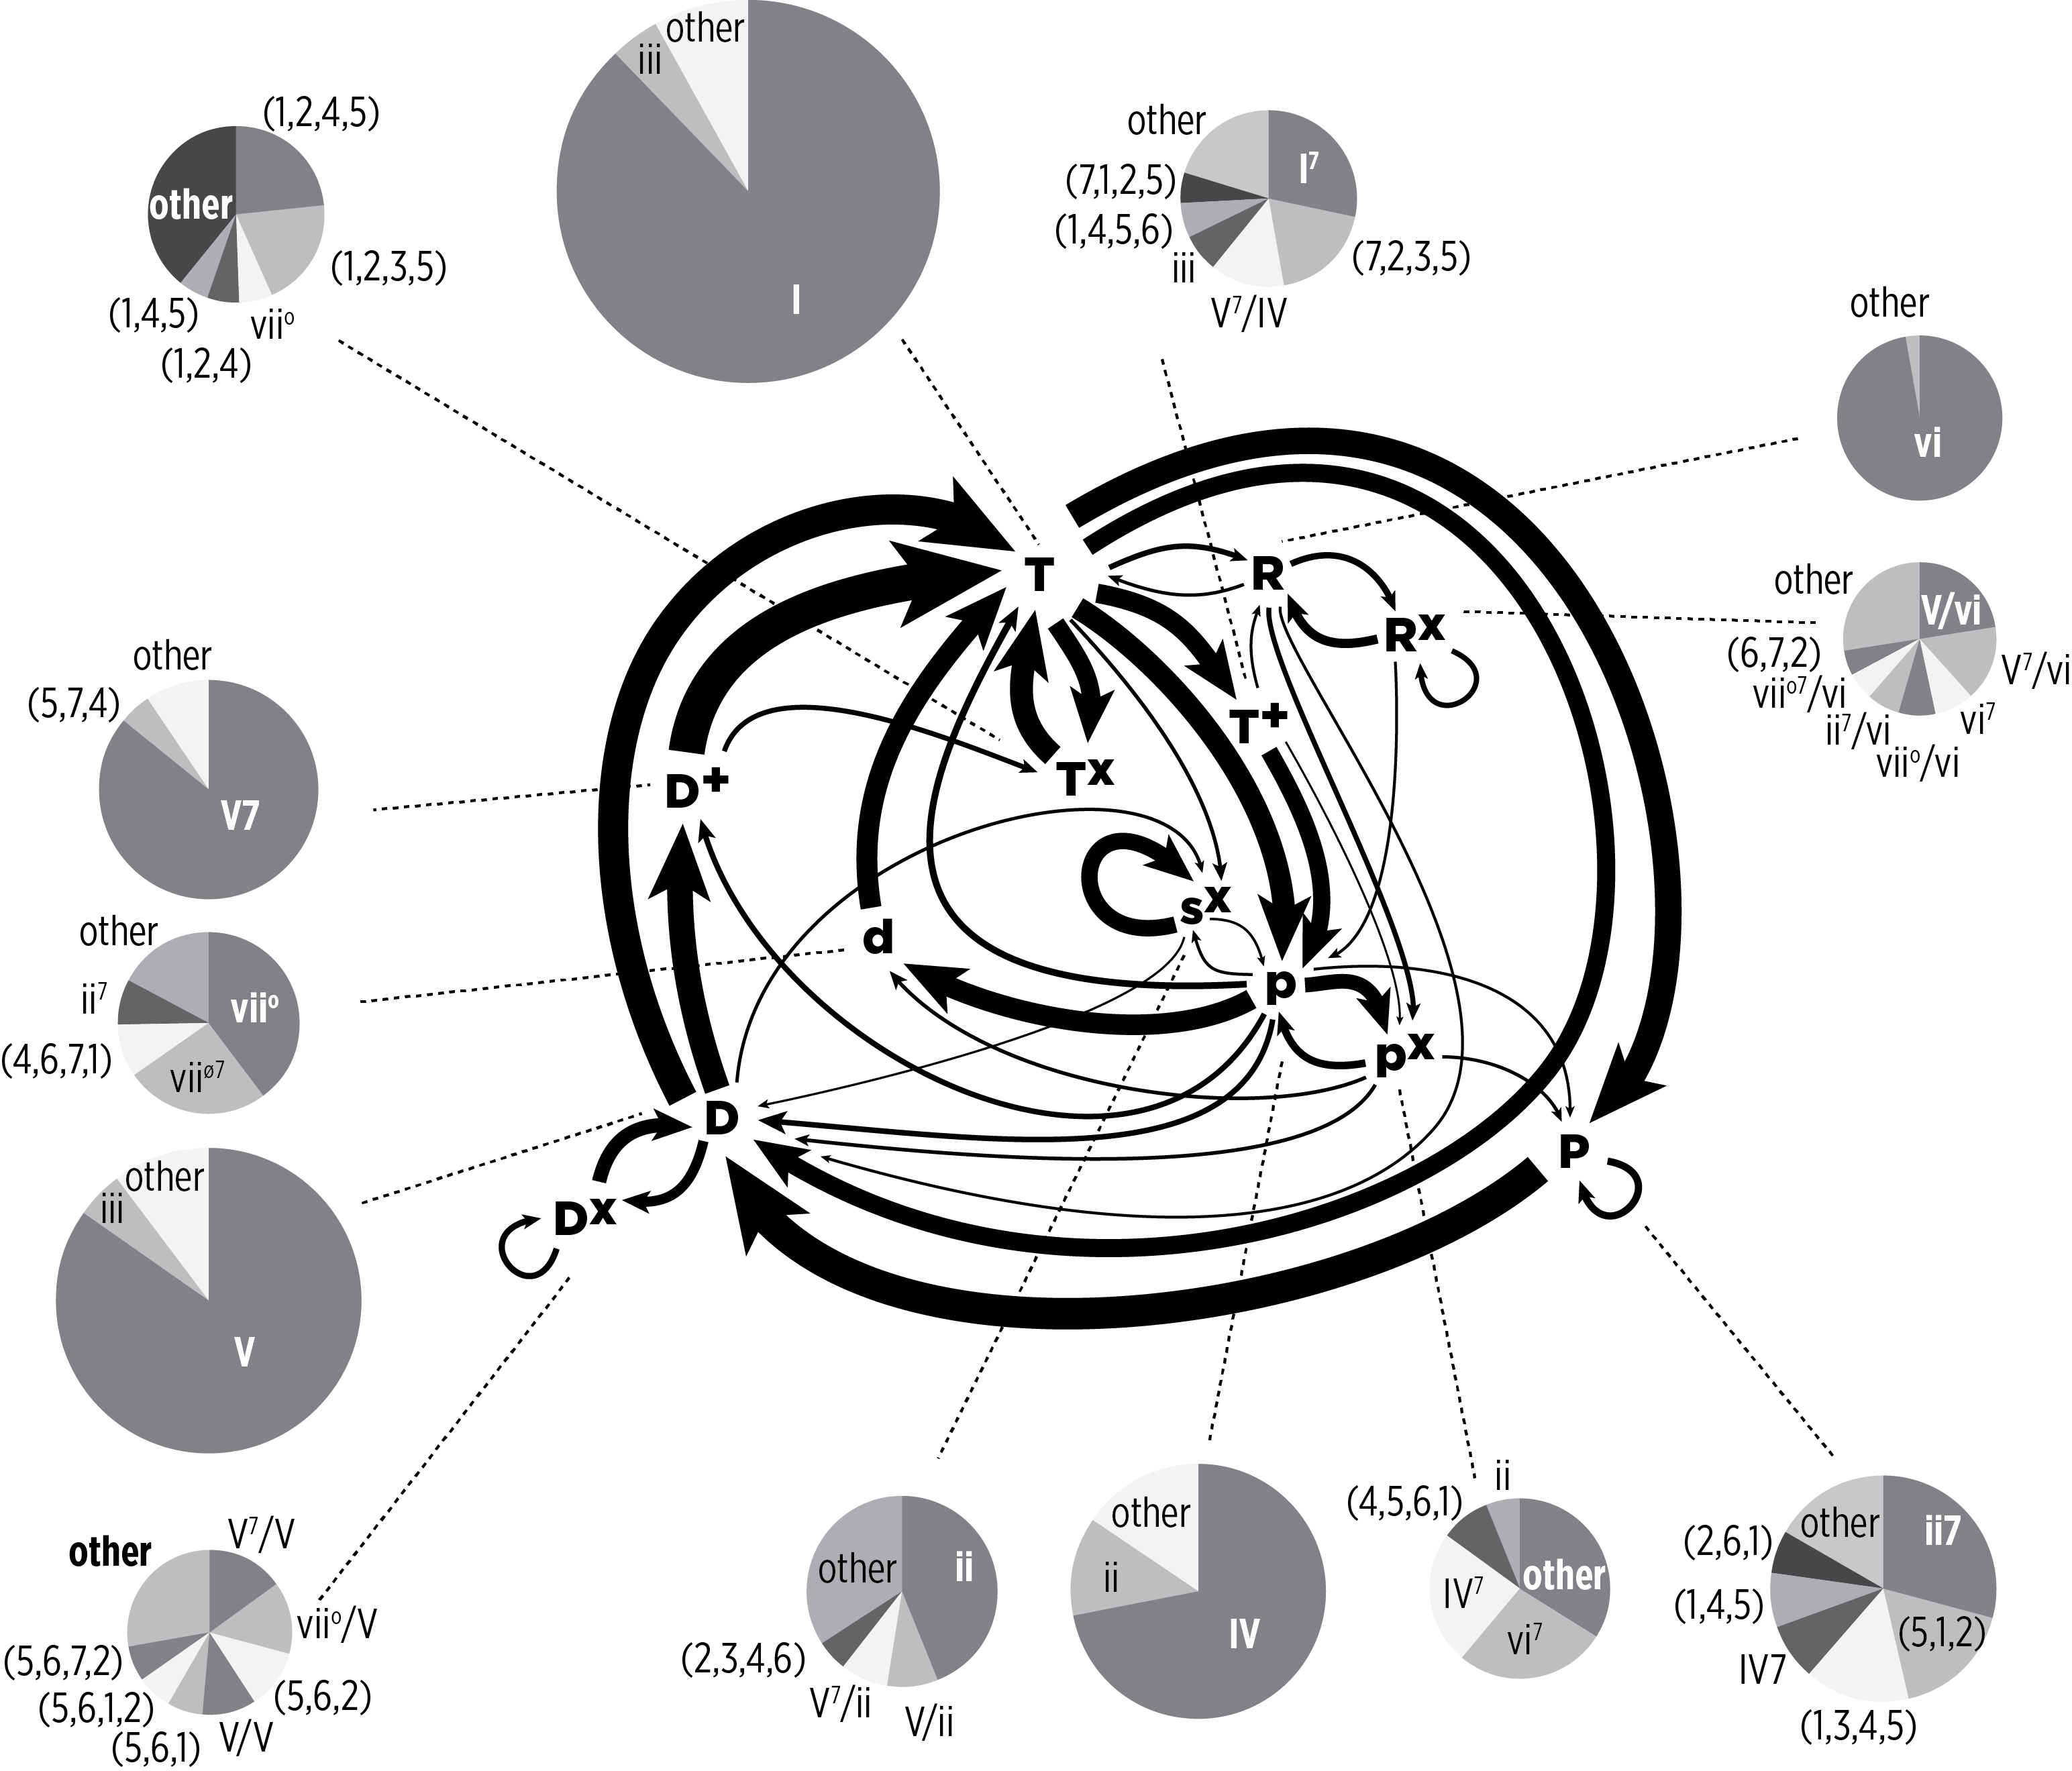
\includegraphics[width=5.5in]{WhiteQuinn_NewPersimmon.png}
	\caption{An empirically-derived ``persimmon" model of functional progression in the Bach chorales, taken from White and Quinn (2016).  Arrows indicate progressions, whether function-preserving (self-progressions) or not (syntactic progressions).  While this diagram encodes progressions on different time scales, neither the progressions nor the functional categories engage with the temporal structure of the data.}
	\label{pers}
\end{figure}

On its most basic level, the ``persimmon" of Figure~\ref{pers} includes a combination of pitch-based chord labels (roman numerals) and functional categories ($T$, $S$, $D$, $P$, and $R$) linked by a variety of arrows.  These arrows indicate common progressions between categories.  Some progressions are from one syntactic function to another -- say, $T \rightarrow P$ or $P \rightarrow D$ -- while others indicate ``self-progressions" like $T \rightarrow T^x \rightarrow T$.  Figure~\ref{iiprog} attempts to show a similar variety of progression types lensed through a more explicit engagement with time.  This chapter will expose the machinery behind and implications of Figure~\ref{iiprog} and its ability to describe multiple \emph{temporal progression regimes} within a single statistical framework.  Examples of short-timespan self-progressions and longer-timespan syntactic progressions will produce chord behavioral curves similar to (but independent of) those in Figure~\ref{iiprog}.  And a consideration of how those curves arise will suggest ways to bootstrap even our types of progression, unearthing different progression regimes directly from the statistical properties of YJaMP's solo piano performances.\footnote{The use of ``bootstrap" here draws on a long computational tradition of responding to a clear problem: if programmatic algorithms generate or load outputs from a series of inputs, how can a system receive the initial impetus to get off the ground?  (For early use of the term in this manner, see Buchholz, Werner (1953). ``The System Design of the IBM Type 701 Computer." Proceedings of the I.R.E. 41 (10): 1273. doi:10.1109/jrproc.1953.274300.)  I hand-supply plausible chord categories here, but I intend this as an initial approximation to be modified later by machine learning methods.}

\section{Chords and Time}
%Chord ``behavior" different on different time scales
%Smallest: static, mostly self-transitions, lends itself to phonetic models
%Small: local behavior, mostly voice-leading neighbors
%Middle: ``Syntactic" models apply, here; suppressions (V-IV) and correlations (V-I)
%Large: predictive power recedes to background statistics (X-...-I)

Temporality and probability lie at the heart of Figure~\ref{iiprog}'s presentation of harmonic progressions.  These two concepts are concretized by the introduction of particular harmonic objects.  In the previous section, the term ``chord category" (applied to $ii$, $V$, and $I$) reflects an artificial (but rather conventional) definition of $ii$ as a category which includes the locally-transposed pitch class sets $[2,5,9]$, $[0,2,5,9]$, and $[0,2,5]$.\footnote{In conventional scale degree terms, these chords are $(\hat{2},\hat{4},\hat{6})$, $(\hat{1},\hat{2},\hat{4}, \hat{6})$, and $(\hat{1},\hat{2},\hat{4})$.  To preserve clarity in chromatic cases and leave enharmonic ambiguities comparatively unresolved, this chapter (and the rest of the dissertation) primarily employs twelve chromatic scale degrees.  While there certainly exist cases where distinguishing between $\flat \hat{5}$ and $\sharp \hat{4}$ is a virtue, both will appear here as $[6]$.}  As seen in Chapter 2, these scale degree sets represent the three most common instantiations of western-classical $ii$ chords found in the YJaMP corpus.  Along similar lines, the $V$ and $I$ categories indicated on Figure~\ref{iiprog} contain ($[2,7,11]$, $[2,5,7,11]$, $[5,7,11]$) and ($[0,4,7]$, $[0,3,7]$, $[0,4,11]$, $[0,3,10]$, $[0,4,7,11]$, $[0,3,7,10]$), respectively.\footnote{The $I$ category combines major and minor mode tonics.  For a discussion of the relative merits of transposing minor key passages with respect to $i$ instead of $vi$, see Chapter 6.}  Machine learning methods will interrogate these chord category assumptions in Chapter 5, but they appear here as the simplest way to connect concepts from traditional harmony to my computational methods.

The horizontal axis of Figure~\ref{iiprog} represents time in consecutive 50-millisecond windows ($w$) -- that is, ``0" is the time at which a $ii$ chord appears, ``1" is 50 milliseconds later, and ``50" is 2.5 seconds (2500ms) after the initial $ii$ chord -- and each point on a given curve indicates how much more or less likely the curve's chord is to be found $w$ windows after a $ii$ chord than it is to be found in the corpus in general.  Some algorithmic detail can help unpack that statement.  Python code finds every instance of a $ii$ chord in the corpus and tallies up everything it finds within the subsequent $w$ windows.  A kind of composite statistical template results: given $ii$ as an ``origin chord," the algorithm returns a probability distribution for each window $w$ in which it accounts for every ``destination chord" found $50w$ milliseconds after a $ii$ chord.  These probability distributions consist of coded versions of claims like ``$w$ windows after a $ii$ chord, chord $x$ appears $y$ percent of the time."  Sorting these window probability distributions produces a list of which chords occur most often at a give time after $ii$ chords.

This list may be interesting in its own right, but it does not make plain the predictive power of $ii$ itself.  A chord highly probable in a window $w$ might reflect a high background \emph{unigram} probability independent of the nearby presence of $ii$.\footnote{For further details on the unigram distribution of the YJaMP corpus, see Chapter 2.}  Figure~\ref{iiprog} normalizes these distributions, however, plotting the difference between two (logarithmic) probabilities on the vertical axis:
\begin{equation}
P(x) = \log_{10} \big( p(x\mid ii) \big) - \log_{10} \big( p(x) \big)
\end{equation}
Here, $P(x)$ is the relative log probability of chord $x$ plotted on the vertical axis of Figure~\ref{iiprog}, while $p(x)$ and $p(x\mid ii)$ are the probabilities of $x$ in the corpus at large and given the previous occurrence of $ii$, respectively.  Subtracting these logarithmic probabilities is equivalent to dividing the probability-given-$ii$ by the probability-in-general outside the logarithmic domain.  The result of the logarithmic normalization is that the positive vertical axis values of Figure~\ref{iiprog} indicate probabilities higher than the background unigram distribution, while negative axis values indicate that the given chord occurs less frequently at a given distance $w$ after $ii$ than it does in the corpus in general -- that the chord is suppressed by $ii$.  Each increase of one unit on the vertical axis corresponds to a particular chord occurring 10 times more probably at a given time window $w$ than its unigram probability.

%talk about using these curves as templates for isolating types of progression behavior into different temporal regimes.
If the curves of Figure~\ref{iiprog} show the relative probabilities of three destination chords, they stand as a way of quantifying the effect of the origin chord ($ii$) on the presence of subsequent $ii$, $V$, and $I$ chords.  The appearance of $ii$ has one particular kind of effect at short distances -- it makes other $ii$ chords much more probable.  But how many chords does $ii$ impact in a similar way, and how many kinds of effect does $ii$ have?

\begin{figure}[h]
	\centering
	\caption{An excerpt of the temporal probability distributions for common chords following $ii$ (unigram-relative log probabilities versus time).  Traditional harmonic theory assumes the ability to reduce this complex temporal data to time-independent category transition rules.}
	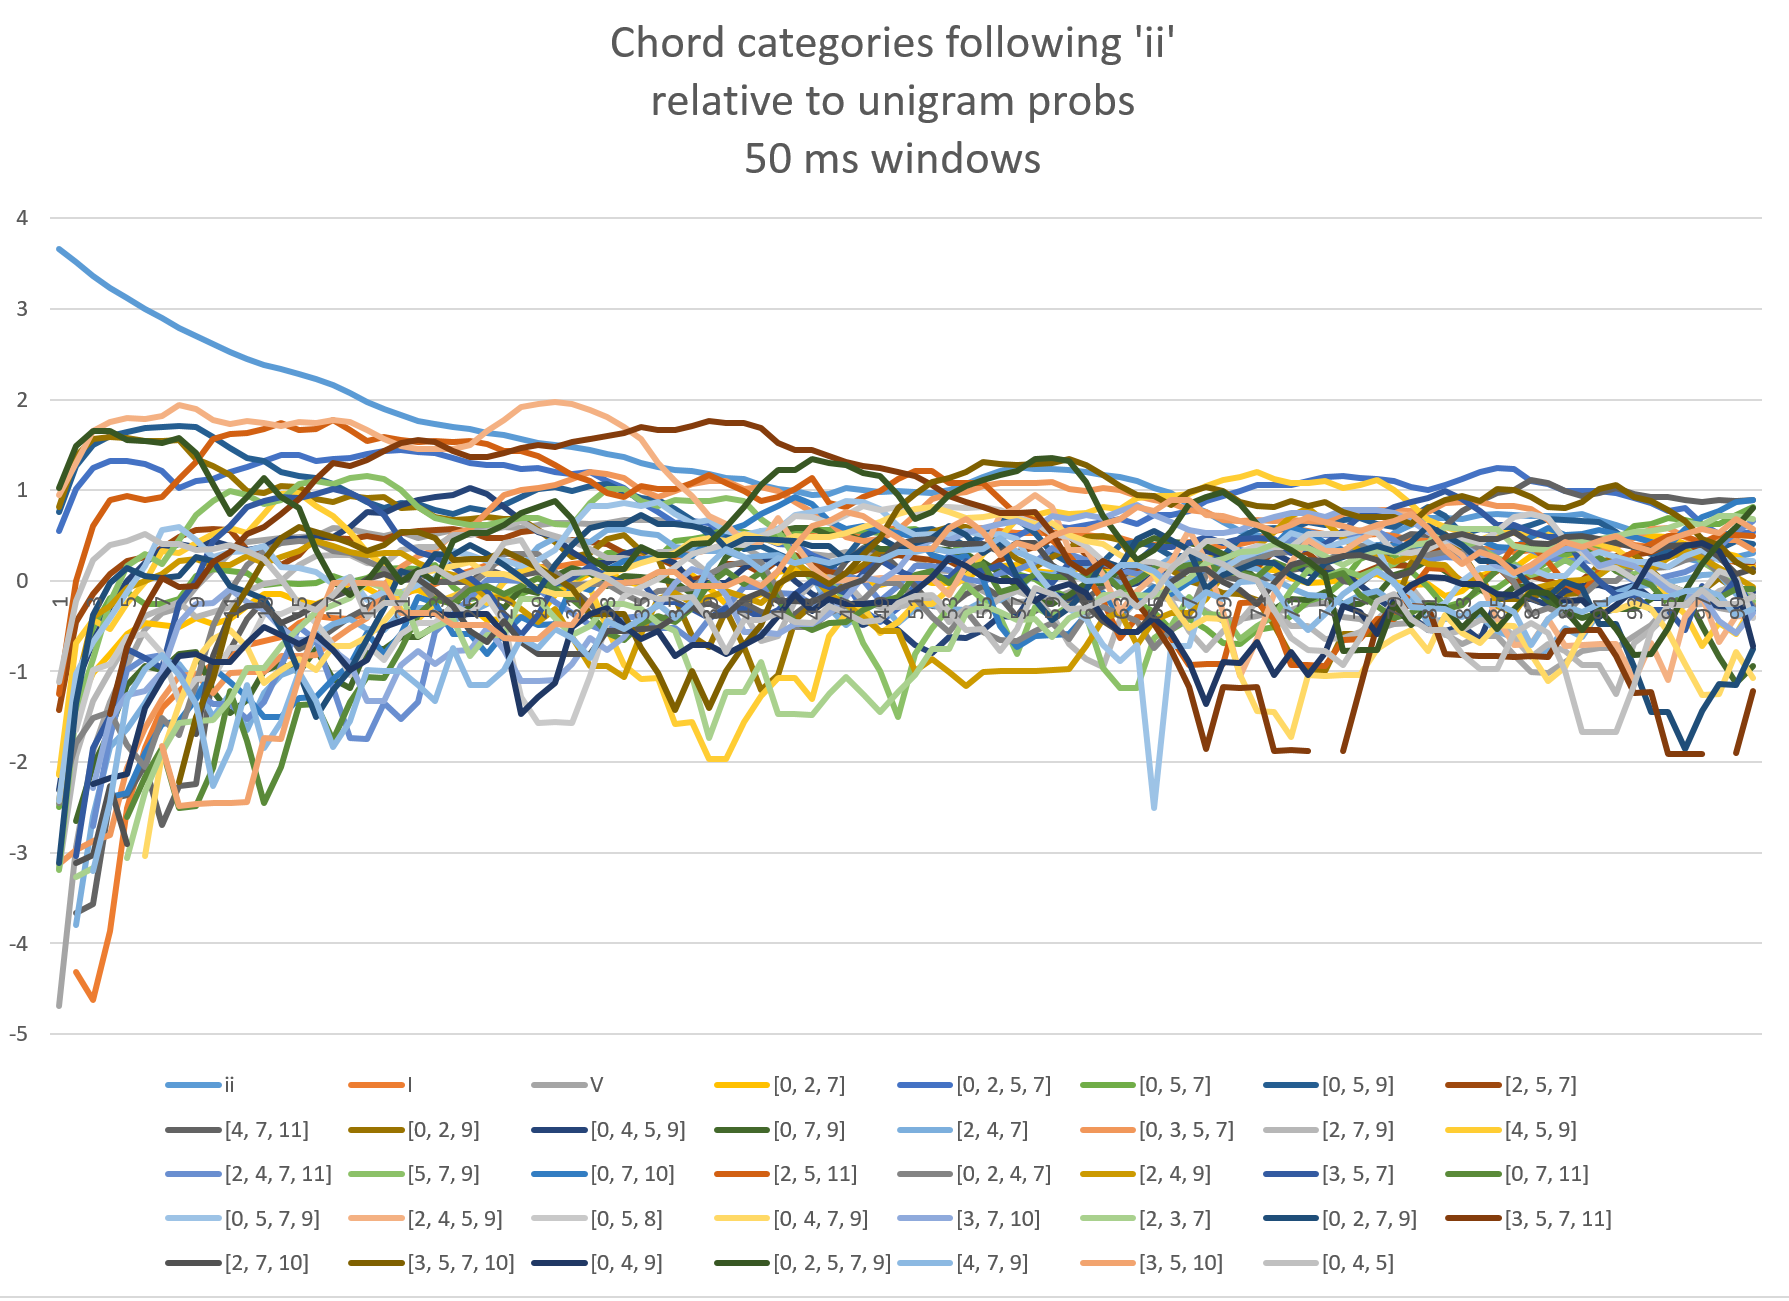
\includegraphics[width=6in]{ii_messy.png}
	\label{ii_messy}
\end{figure}

Figure~\ref{ii_messy} combines a small fraction of the destination chord distributions for chords following $ii$.  Many high-probability origin chords in the corpus have more than 1000 distinct destination chords within 100 50ms windows.  Sorting through these distributions by hand is not feasible, and many of the destination chords are low-probability objects in the first place; there is no guarantee that random fluctuations in the appearance of rare chords will tell us anything about $ii$'s syntactic properties.

Thankfully, to find other chords strongly impacted by $ii$ in ways similar to the behavior displayed in Figure~\ref{iiprog}, it suffices to compare the large number of destination chord probability distributions to those of $ii$, $V$, and $I$.  Curves which lie close to the $V$ curve correspond to chords with behavior similar to $V$.  This sounds tautological, but an important distinction is at play: a chord with a temporal probability distribution similar to that of $V$ on Figure~\ref{iiprog} may have absolutely no discernible pitch relation to $V$ as a scale degree set.  ``$V$-like" chords, distributionally speaking, need only \emph{act like} $V$, statistically, in the presence of $ii$.  In other words, calculating which destination chord probability distributions lie closest to those shown in Figure~\ref{iiprog} picks out chords which display behavior similar to self-progressions and syntactic progressions.  This easily automated process assembles chord progression categories on more than one time scale -- and it can be performed for any origin chord.

\section{Phonetic scale}
On the shortest of musical time scales, the $ii$ chord tends to predict itself quite strongly, and it does so with diminishing strength as time passes.  To find what other chords behave this way after the appearance of $ii$, a few lines of code iterate across all of the observed destination chord distributions.  For each destination chord $d$, the code sees an $n$-dimensional probability vector, where $n$ can range up to the value of $w$ corresponding to the maximum time delay for which statistics are kept.  It compares this vector to the $n$-dimensional ``self-progression" prototype (the $ii$ distribution) element-wise, subtracting the log probability of the current destination chord ($p_d$) from the log probability of the $ii$ chord ($p_{ii}$) at each window location.  Summing the absolute value of all of these deviations gives a simple metric for how dissimilar the destination chord is from $ii$:
\begin{eqnarray}
p_{ii} &=& (x_1, x_2, ... ,  x_n) \\
p_{d} &=& (y_1, y_2, ..., y_n) \\
D_{(ii,d)} &=& \sum_{w=1}^{n} \lvert y_w - x_w \rvert
\end{eqnarray}
That is, the code subtracts the probability of the origin chord $ii$ in window 1 from the probability of the destination chord $d$ in window 1, takes the absolute value of the difference, and combines the resulting distances over some $n$ consecutive time windows.  Setting $n$ is a matter of taste; I have chosen here to compare curves out to where the behavior of the prototype begins to level off.  For the self-progression $ii \rightarrow ii$, Figure~\ref{iiprog} suggests $n=40$ as a reasonable cutoff, though employing similar values yields similar results.  Minimizing dissimilarity $D_{ii,d}$ provides a list of the destination chords which best fit the short-term behavior of $ii$.  A plot of the 5 best destination chords of this type is given in Figure~\ref{ii_phonetic}.

\begin{figure}
	\centering
	\caption{The 5 destination chords for $ii$ progressions with temporal probability distributions most similar to that of $ii$ (unigram-relative log probabilities versus time).}
	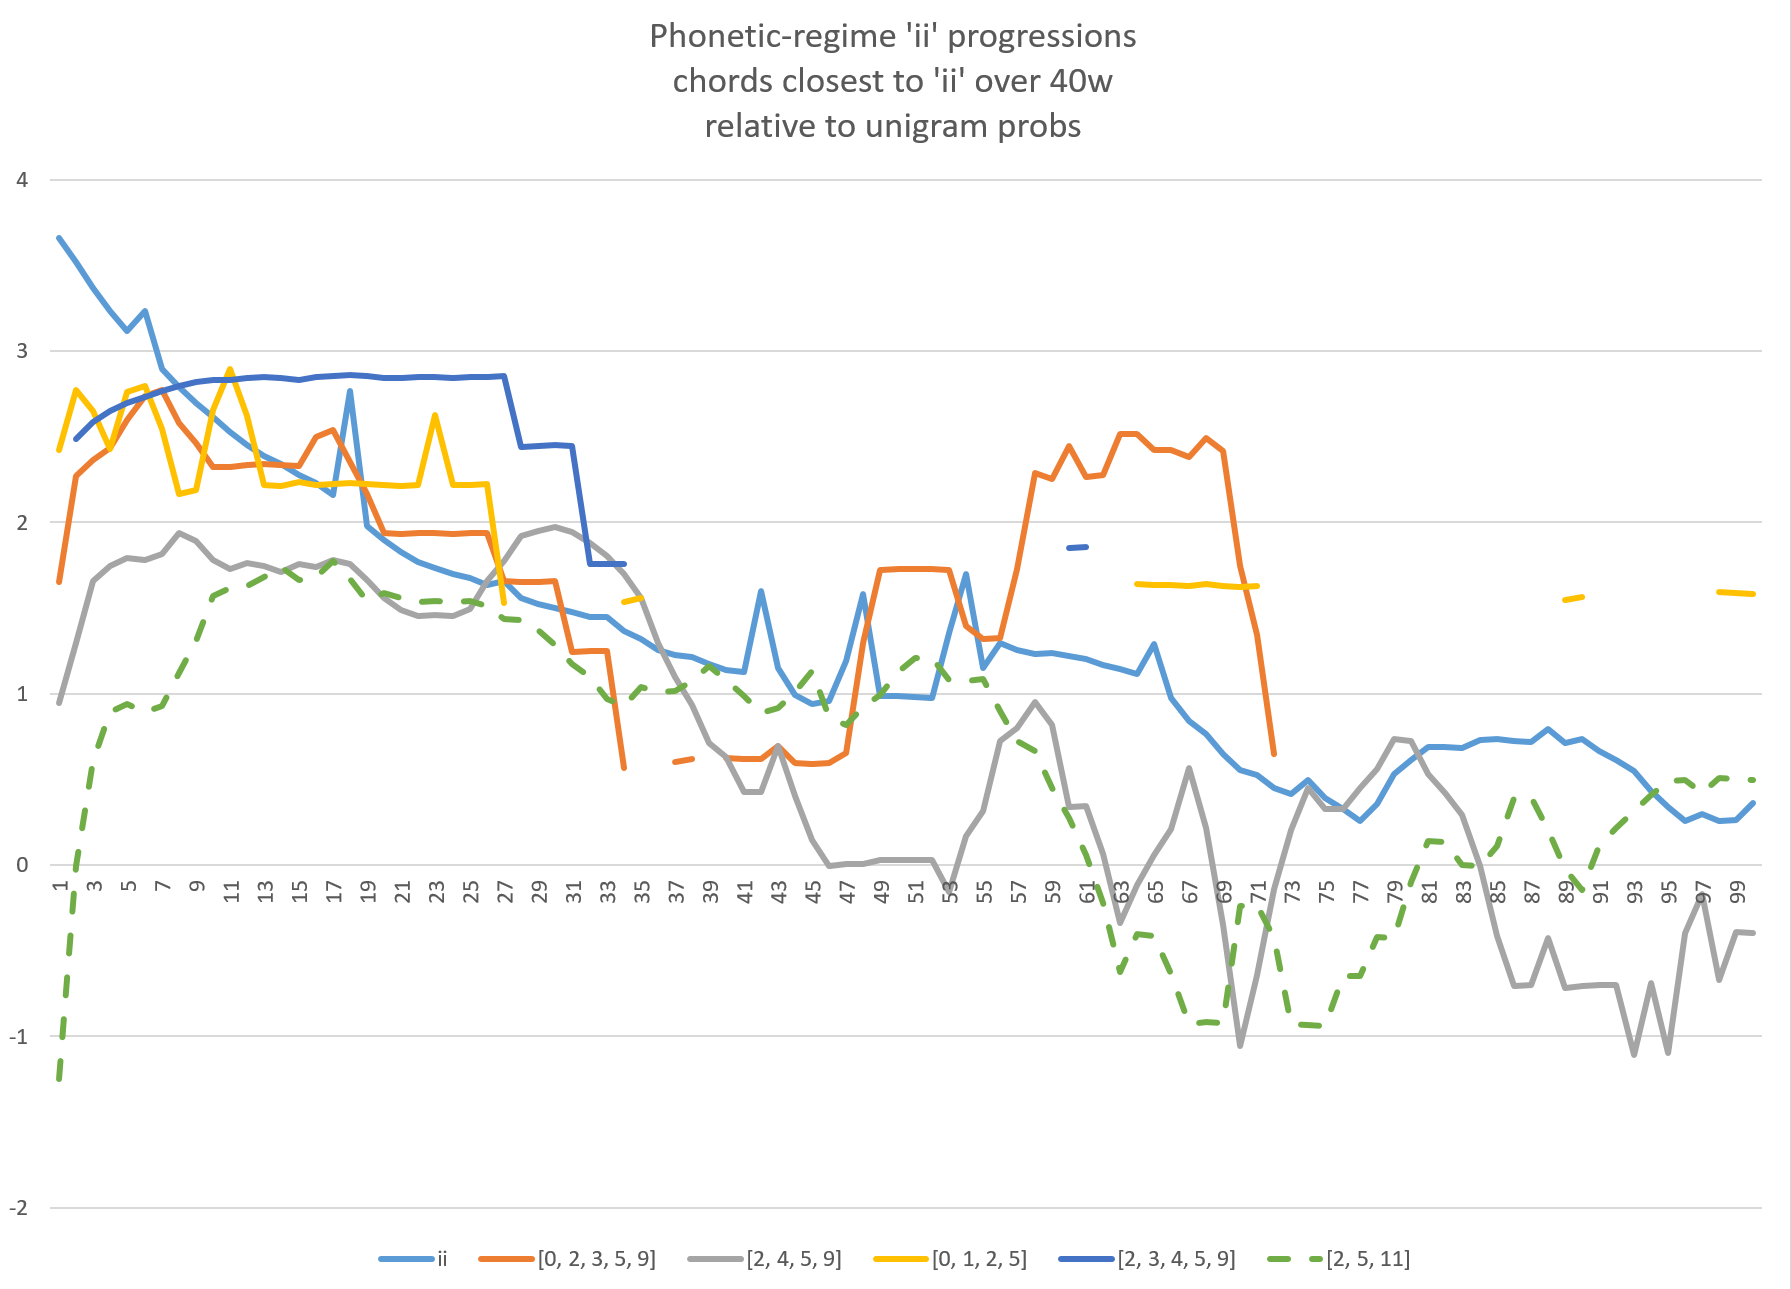
\includegraphics[width=6in]{ii_phonetic.png}
	\label{ii_phonetic}
\end{figure}

The results are striking in their predictability.  While pitch class/scale degree content played no role in the selection of self-progression destinations for $ii$, most of the destination chords with behavior most similar to $ii$ consist of some form of $ii$ chord with one or more added tones. $[0,2,3,5,9]$ and $[2,4,5,9]$ likely draw scale tones from their minor and major tonics, respectively, while $[0,1,2,5]$ and $[2,3,4,5,9]$ appear to arise from some local melodic motion.  In general, the list of self-progression partners for $ii$ suggests two rough categories of behavior:
\begin{enumerate}
	\item The destination chord may be related to the origin $ii$ chord by harmonic or quality completion.  Example: $[0,2,5] \rightarrow [0,2,5,9]$.
	\item The destination chord may be related to the origin $ii$ chord by the introduction of melodic notes. Example: $[0,2,5,9] \rightarrow [0,2,3,5,9]$.
\end{enumerate}
The two types of behavior can be combined, and there are also conditions where a self-progression may ambiguously result from either (i.e., $[2,5,9] \rightarrow [0,2,5,9]$).  More detailed statistics regarding the particular scale degree sets and voicings participating in these progressions can be gleaned from combining these observation with the unigram-labeling methods of Chapter 2.

In general, few of the progressions at this time scale consist of transitions which an analyst would deem sufficient to indicate a change of ``chord" or ``function."  Moreover, several self-progressions consecutively might be necessary to fill out all the pitches implied by an analyst's roman numeral.  As a result, I refer to this temporal progression regime as the \emph{phonetic regime}, by way of analogy to linguistics.  In the way that multiple phonemes might make up a word, multiple self-progressions in this regime might make up a functional chord, and the particular ways in which phonetic regime chords are connected to one another rely on particular choices of voicing and melodic context in much the same way that the surface-level phonetic traces of linguistic syntax depend on the particulars of word order and nearby syntactic partners.\footnote{I feel certain that the phonetic analogy with musical chord fragments does not originate with me, but I have yet to find a smoking gun.  Until someone enlightens me, I will continue hunting for throwaway comments made by Ray Jackendoff.}  If harmonic syntax is to include primarily progressions from one function to another, then the phonetic regime provides a clean and empirically-grounded sense of the morphological transformations necessitated by concatenating syntactic partners.

So far, I have avoided mentioning the fifth most $ii$-like member of the (fuzzy) phonetic progression regime, shown in Figure~\ref{ii_phonetic}: $[2,5,11]$.  This chord, usually labeled $vii^{\circ}$, is not typically said to have the same function as $ii$.  Its presence on the plot might imply two things: that $[2,5,11]$ may appear as a phonetic neighbor to a more normative $ii$ chord (like $[2,5,9]$), or that destination chord curves this far below the self-progression $ii$ prototype begin to behave more like syntactic progression destinations than phonetic ones.  The $[2,5,11]$ distribution of Figure~\ref{ii_phonetic} falls almost exactly midway between the prototype curves for $ii$ and $V$ on Figure~\ref{iiprog}, and its behavior in different contexts might suggest assigning it a dual status, playing a role in the phonetic and syntactic regimes.

In any event, chord category formation involves much more than a quick perusal of Figure~\ref{ii_phonetic}.  Comparing destination chord regimes across many origin chords provides a much broader data set better suited to machine learning techniques.  Example phonetic and syntactic regime plots for origin chords other than $ii$ are included at the end of this chapter, and the integration of these disparate distributional portraits with machine learning is left to the next chapter.

\section{Local syntactic scale}
Finding syntactic progressions amounts to a change in time scale.  The previous section showed that self-progression destination chords could be found by calculating which distributions most closely resembled $ii\rightarrow ii$ over short time scales, regardless of pitch content.  The same logic applies to functional syntactic progressions: if $ii\rightarrow V$ is a prototypical syntactic progression, syntactic regime destination chords should have temporal probability distributions similar to that of $V$ over moderate time scales.  Judging from Figure~\ref{iiprog}, that time scale is about $60$ time windows, or 3 seconds.\footnote{Here, again, I choose the time scale cutoff rather intuitively, assuming that the initial suppression, sharp increase in probability, and return to unigram probability are all features of syntactic-$V$-ness.  It is unclear to me, however, if the lower-probability fluctuations at the end of the temporal tail bear important information.}  The best-fitting curves appear in Figure~\ref{ii_syntactic}.

\begin{figure}
	\centering
	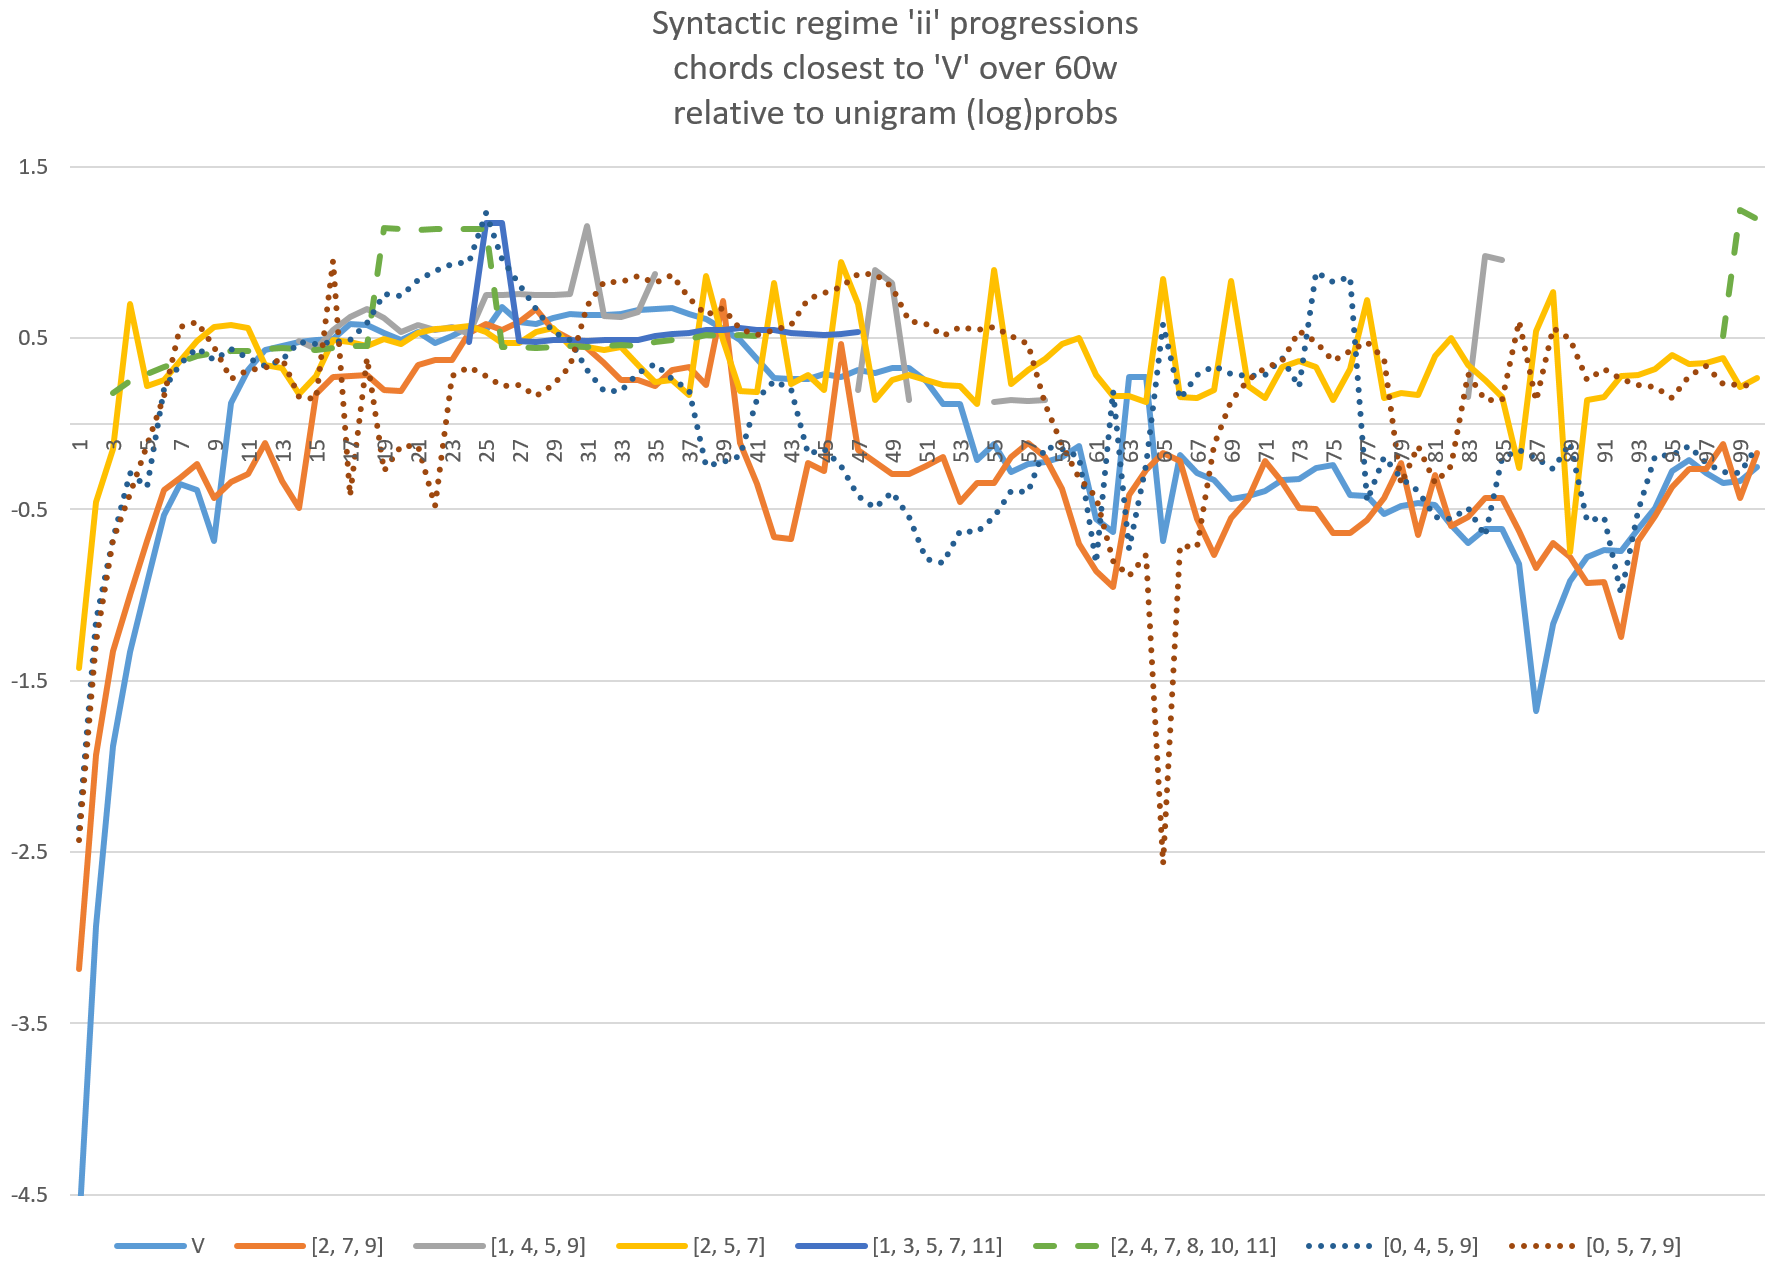
\includegraphics[width=6in]{ii_syntactic.png}
	\caption{The 7 destination chords following $ii$ with syntactic regime probability distributions most closely resembling that of $V$.  Chords similar to both $V$ and $IV$ appear to behave similarly.}
	\label{ii_syntactic}
\end{figure}

Many of the destination chords which most closely resemble $V$ in this context are chords we might think of as phonetically-related to $V$ proper.  $[1,3,5,7,11]$ can be parsed as a $V^{\sharp 11 \flat 13}$, and $[2,5,7]$ may function as an incomplete $V^7$.  $[2,7,9]$ might be related to $[2,7,11]$ by melodic step, or it could be a symptom of more complicated behavior in play; $[2,4,7,8,10,11]$ is almost certainly the latter.  But the syntactic nature of the $V$ curve does more than pick out its own phonetic neighbors.  Since no pitch class or root similarities are assumed, behavioral similarity also strongly selects another type of chord likely to follow $ii$: $IV$ chords.  Shown in the dotted curves of Figure~\ref{ii_syntactic}, $[0,4,5,9]$ and $[0,5,7,9]$ are both likely to follow $ii$ in a way similar to $V$ -- both types of chord would be deemed syntactic if found a moderate time after $ii$.

In this way, syntactic regime progression data partly reproduces and partly cuts across traditional functional harmony expectations.  Crucially, not all chords which behave like $V$ after $ii$ \emph{always} behave like $V$.  Each possible origin chord provides a distinct set of phonetic and syntactic data to be used for functional categorization.  The $ii$ syntactic data here indicates a category of ``chords which follow $ii$ at moderate delays," of which both $IV$ and $V$ are members, but other syntactic data might distinguish the two.  Before Chapter 5 attempts to address this inductive category formation problem, it is worth asking another difficult inductive question directly: how many temporal syntactic regimes are there, and can they be extracted from the data without assuming prior prototypes?

\section{Temporal Progression Regimes}
The selection of $ii$, $V$, and $I$ as prototypes for categories of temporal progression behavior served an important purpose.  Since probabilistic statistics connect each origin chord to a large number of destination chords, some principled method for selecting destination chords with common behaviors is necessary.  The examples used in this chapter depend on thousands of 100-dimensional vectors, each of which features its own unique shape.  Choosing temporal progression prototypes constitutes a selection of shape types.  I assumed that the shapes of the $ii$, $V$, and $I$ chord distributions (when following a $ii$ origin chord) were common and important ones.  But the data can suggest its own collection of shape types.

Principal component analysis (PCA) treats problems of exactly this nature in the world of machine learning.\footnote{Common in the machine learning literature, PCA first appears in Pearson, K. (1901). "On Lines and Planes of Closest Fit to Systems of Points in Space." \emph{Philosophical Magazine} 2 (11): 559�572.  Other machine learning techniques accomplish similar ends, and I have no proof that PCA provides optimal results -- but it does provide results.}  Given a data set with a high-dimensional coordinate basis -- like a set of 100-dimensional vectors -- PCA constructs a lower-dimensional coordinate system, projecting elements of the data set onto new basis vectors which best account for a maximum amount of the variance in the data.  The details are complex, but some broad-strokes intuitions help contextualize the results of interest.

To cast the destination chord probability distributions into a form amenable to PCA, it helps to think of each distribution as a single point in a plot with 100 axes -- one corresponding to each time window. In schematic form, PCA then asks a series of questions about this noisy cloud of temporal probability distribution points:
\begin{enumerate}
	\item How do the data points (destination chord distributions) vary with respect to each of the 100 (temporal) basis coordinates?
	\item Are the distributions at any combination of axes (that is, time coordinates) correlated with one another?
	\item Along what direction in this 100-dimensional space is the largest variance in the data?  If a non-trivial set of time coordinates frequently indexes correlated probability values, that direction may not be along a single one of the 100 axes.
	\item Can a small number of such directions reasonably capture the majority of the variance in the data?  If so, re-label the data in terms of those directions, rather than the original 100 axes.
\end{enumerate}

The first two questions ask if the behavior of destination chords at, say, 50 milliseconds tends to be correlated with their behavior at some other time(s).  Most of the temporal probability distributions extracted from YJaMP are quasi-continuous -- the probability of $V$ at time point 4 is likely to be close to the probability of $V$ at time point 3 -- which means that consecutive time points tend to index similar probability values for a given destination chord distribution.  In the ``cloud of points" frame of reference, this means that a distribution with a high value along axis 4 is relatively likely to have a similarly high value along axes 3 and 5. The probability at consecutive time points is likely to be positively correlated.  Alternately, destination chord distributions with high probability values at very short distances may tend to have low probabilities at long distances, or vice versa, producing negative correlation.  In either case, correlated temporal probability data exists in the distributions over their time coordinate basis.

The third question asks if a particular direction in the cloud of points can capture a large swath of the data.  If the destination chord probability distributions were identical at all time scales except for the very first window, this question would be trivial: the direction of the first axis would account for \emph{all} of the variance in the data, and a new set of coordinates could discard 99 of the axis variables without losing any information about differences in the distributions.  But for the actual YJaMP progression data, the distributions usually vary over all 100 time scales, many of which are non-trivially correlated.  It might be that chords in the phonetic regime primarily vary over windows 1-20, and that the variance in each of those windows is strongly correlated.  If those variances are similar, a PCA algorithm will select as a basis vector some linear combination of the original axes that is maximally aligned with the direction of variance.

The fourth question ensures that the variance-maximizing basis vectors are produced in descending order of variance capture.  Each of the first few newly-calculated axes -- principal components -- can be used to describe a large amount of the data. Crucially, after the first few components, PCA enables the analyst to stop tracking dimensions while losing a minimal amount of information regarding the differences between the data points.  Instead of searching for patterns in all 100 time variables of the figures above, PCA focuses on a small number of new dimensions.

All of these machinations produce two positive outcomes: First, these new components form a coordinate system in which the destination chord probability distributions have radically simpler coordinates -- only a few numbers, instead of 100.  And secondly, the resulting components provide templates for the ways in which categories of destination chord distribution differ from each other most significantly.  They provide automated, data-driven indications as to how many different temporal progression regimes there might be, and they present shape types indicative of the types of variance to expect.

Running PCA on the large number of destination chord probability distributions decomposes the high-dimensional time-based coordinates into a low-dimensional basis of temporal progression regimes.  The first 5 machine-generated principal components for $ii$ chord destinations are plotted in Figure~\ref{ii_pca}.
\begin{figure}
	\centering
	\caption{The top 5 principal components calculated from the full set of destination chord temporal probability distributions following $ii$.  The plot is of probability versus time; the legend indicates the components and their variance percentages in descending order.}
	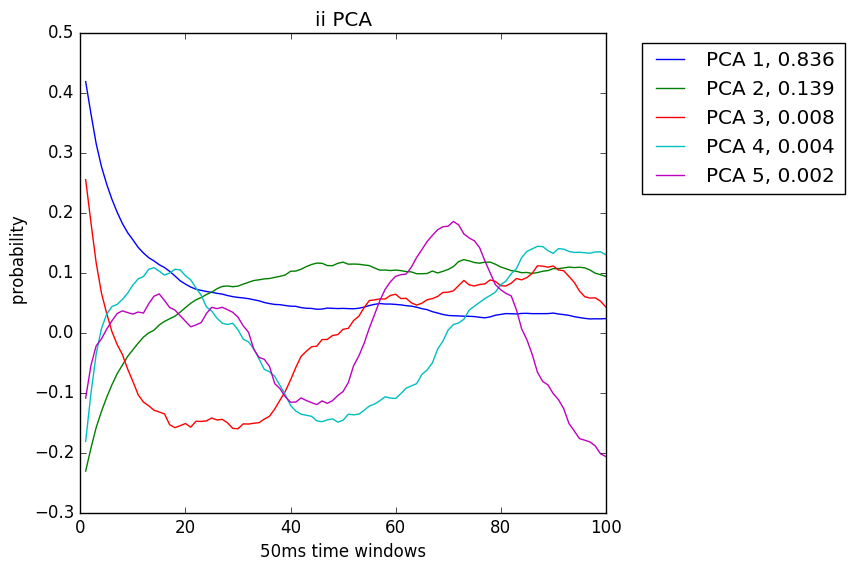
\includegraphics[width=6.5in]{iipca_ABS.png}
	\label{ii_pca}
\end{figure}

With slight theoretical adjustments, I propose that these distribution shape classes (or, more properly, combinations thereof) can be used in place of the hand-picked $ii$, $V$, and $I$ shape templates employed earlier in the chapter for the assembly of phonetic and syntactic progression regimes.  The first principal component, the blue curve on the figure, accounts for most of the variance in the distributions; high and low scores with respect to this component indicate behavior where the shorter time spans vary much more than the longer ones, behavior comparable to that of the phonetic regime.  Component 2, the green curve, corresponds to chords initially suppressed but predicted later, similar to the behavior of chords in the syntactic regime.  Components 3-5 indicate more nuanced variance behavior, but they only account for a very small percentage of the data's variance: the lion's share of information is captured by the first two components, providing strong motivation for the existence of precisely two progression regimes -- the phonetic and the syntactic.

These machine-generated regimes of chord behavior provide a framework subsuming both ``embellishing" and ``harmonic" progressions -- a general statistical model of temporal progression behavior.  They rely on no particular knowledge regarding the pitch content of the chords involved, and they suggest both the number of regimes and their characteristic shapes empirically.  They provide a proof of concept that progression types for a given origin chord (in this case, $ii$) can be learned from complex data with minimal assumptions.  Extending this information to a variety of origin chords and inducing a grammar through machine learning are left to the next chapter.

\newpage
\section{Other Origin Chords}

%dump, for now
\begin{figure}[h]
	\centering
	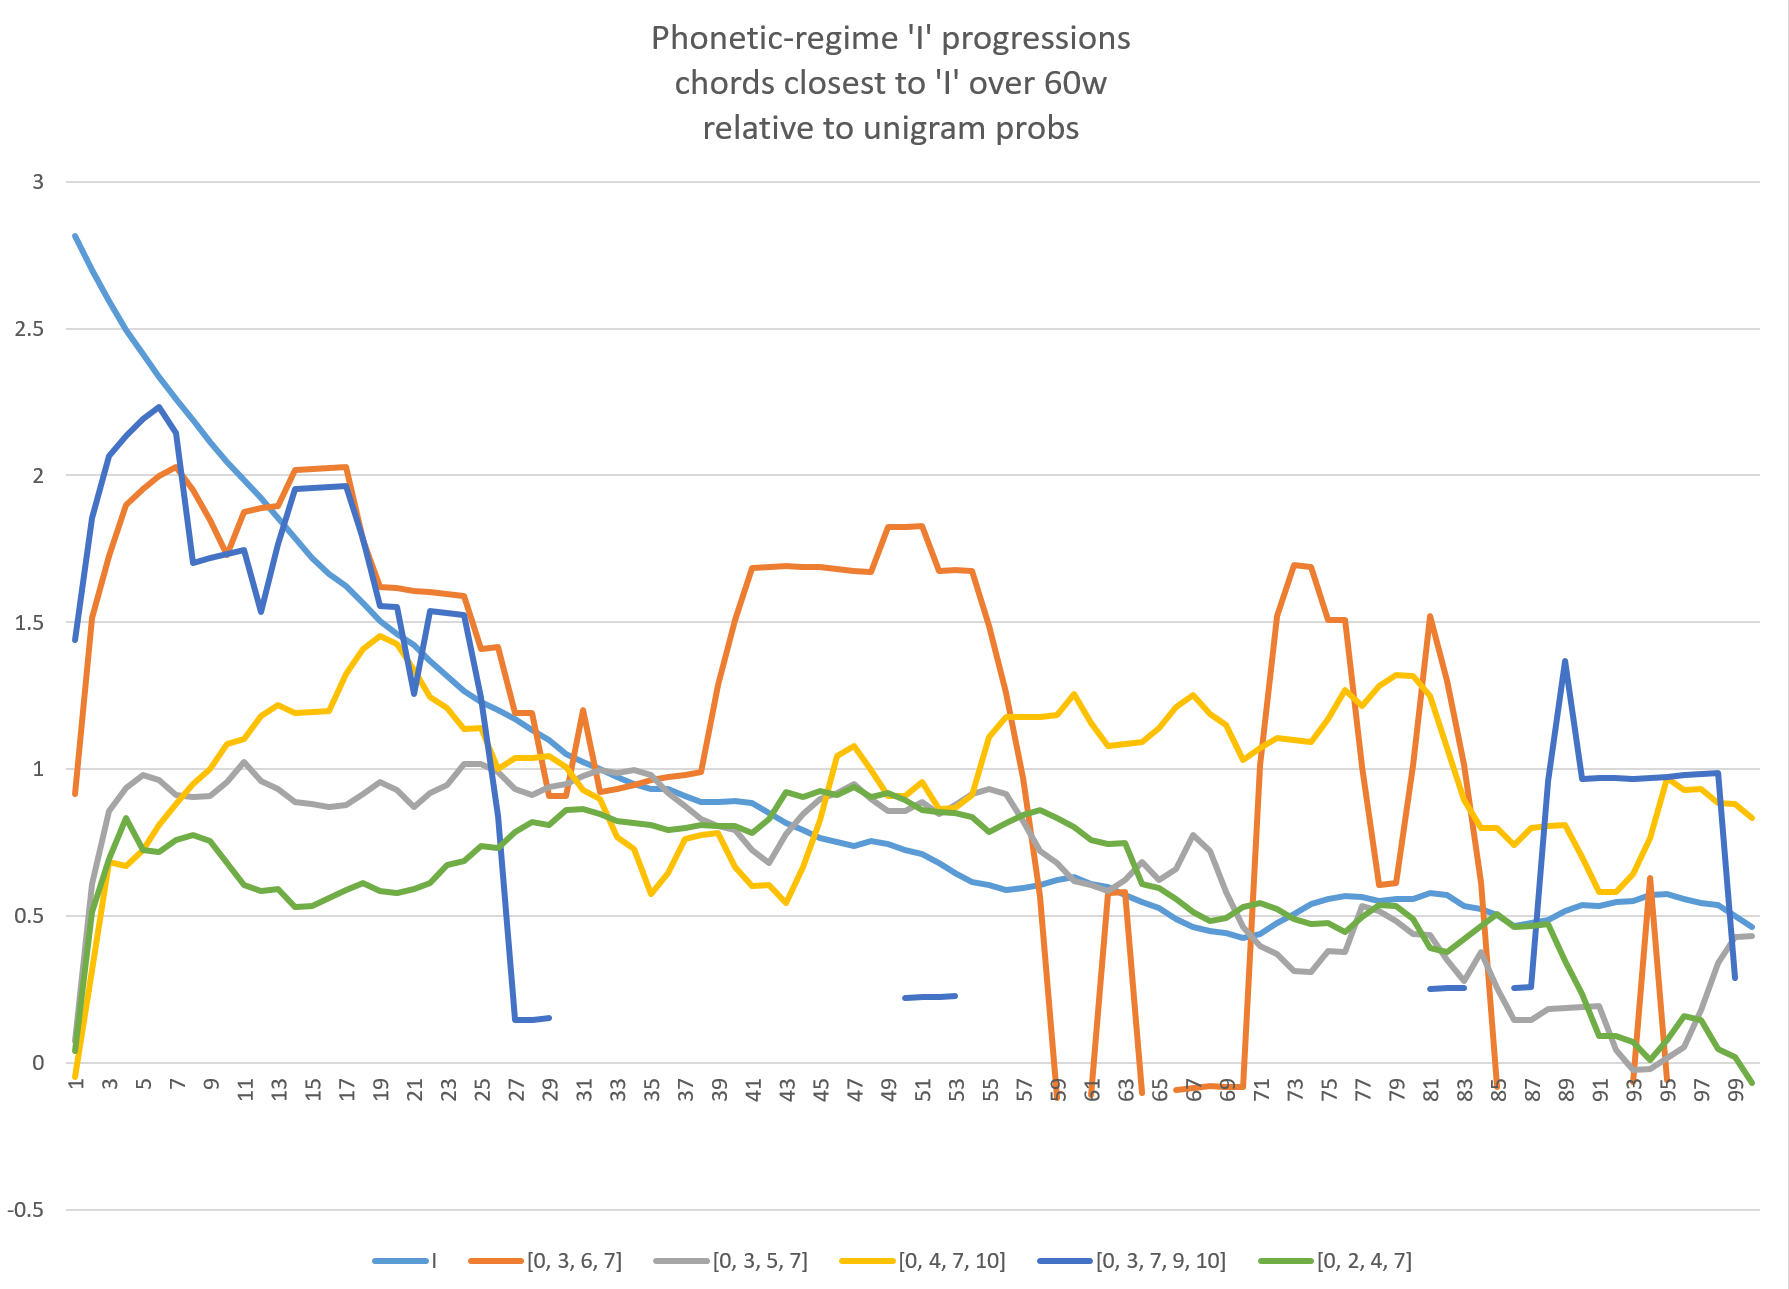
\includegraphics[width=6in]{I_phonetic.png}
	\caption{Phonetic regime self-progression destination chords following the appearance of $I$.}
	\label{I_phonetic}
\end{figure}

\begin{figure}[h]
	\centering
	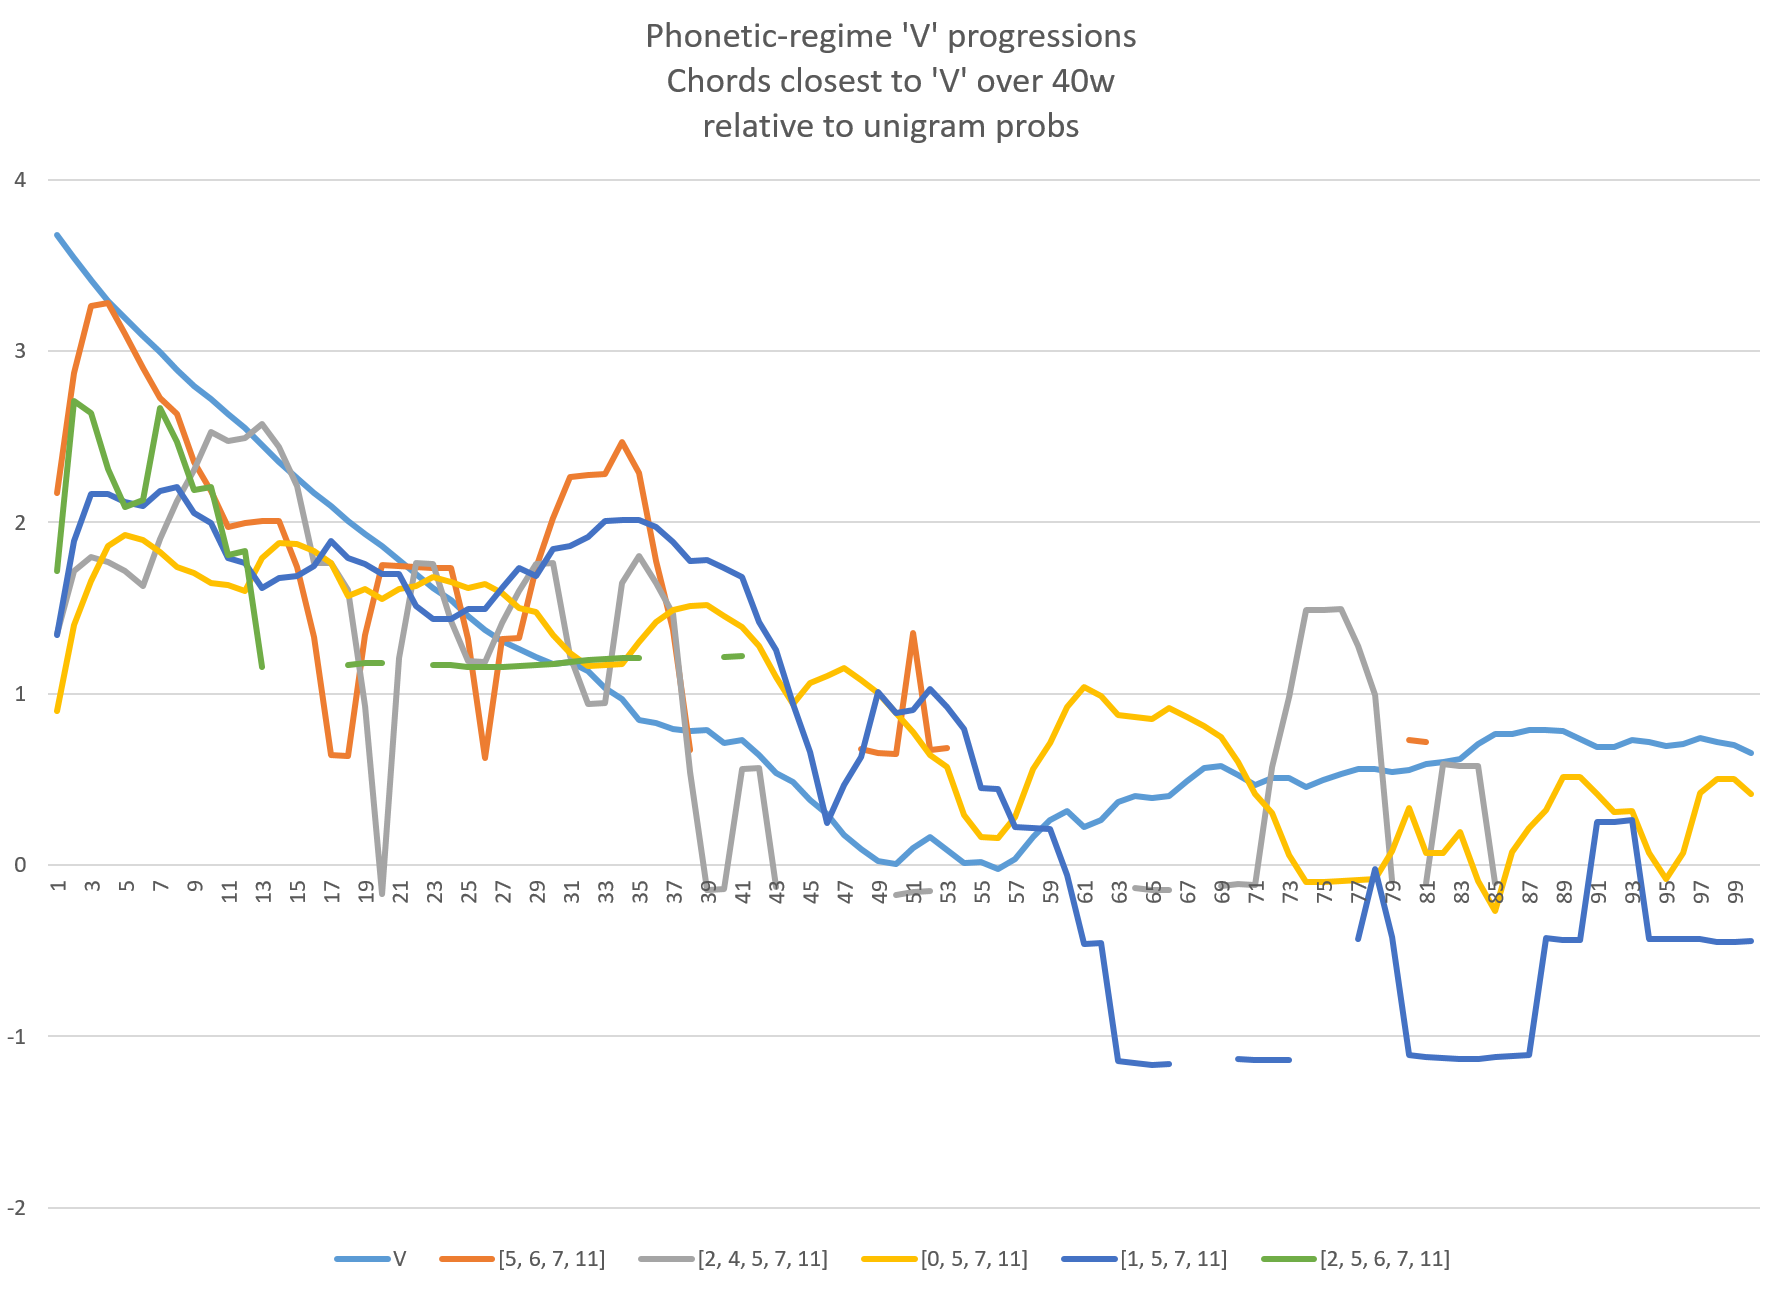
\includegraphics[width=6in]{V_phonetic.png}
	\caption{Phonetic regime self-progression destination chords following the appearance of $V$.}
	\label{V_phonetic}
\end{figure}

\begin{figure}[h]
	\centering
	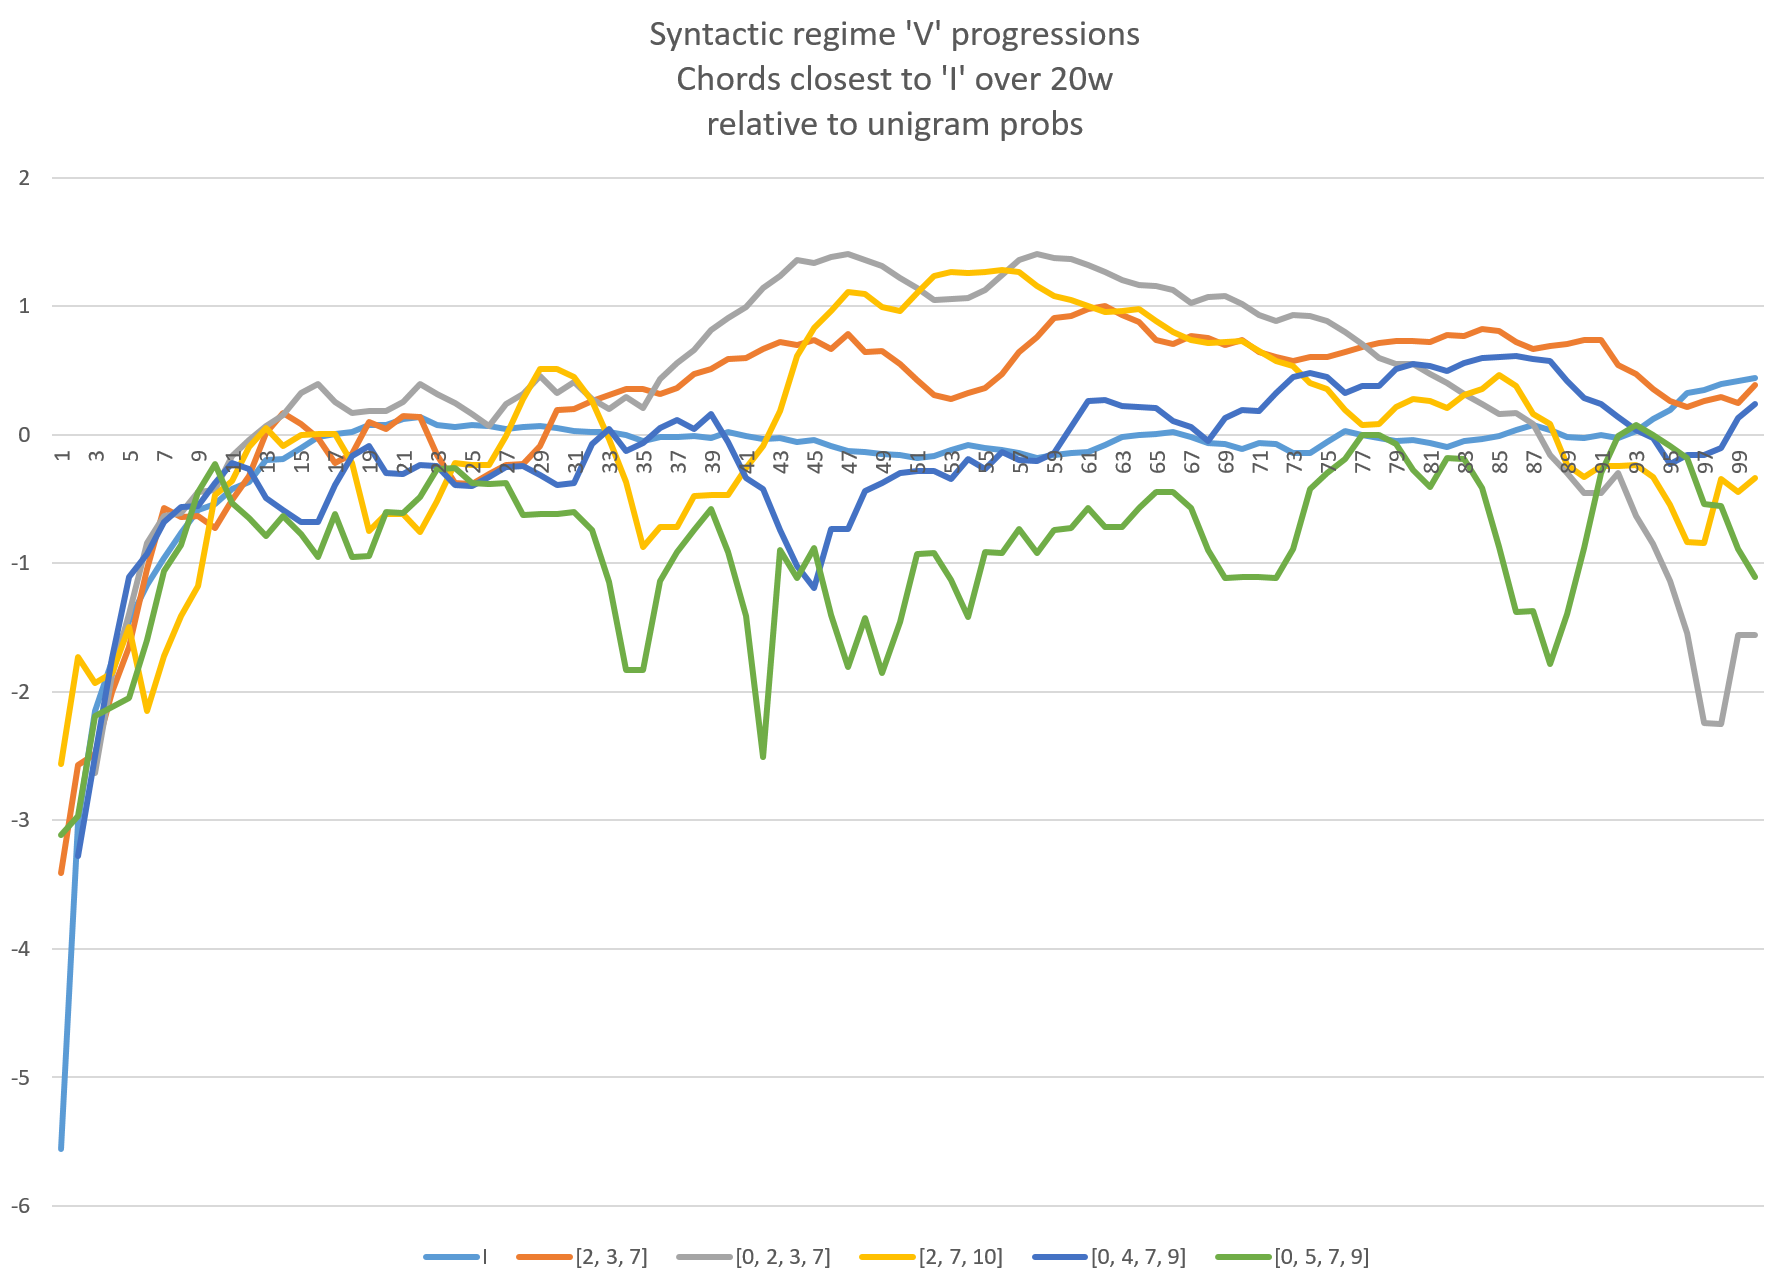
\includegraphics[width=6in]{V_syntactic.png}
	\caption{Syntactic regime destination chords following the appearance of $V$.  Note the comparatively short time delay; $V$ does not have a strong predictive impact on the appearance of $I$ for very long.  This is likely due both to the very high unigram probabilities of $I$ and $V$ and to $V$'s role in faster progressions (compared to $ii$).}
	\label{V_syntactic}
\end{figure}
